\documentclass{standalone}
\usepackage{tikz}
\begin{document}


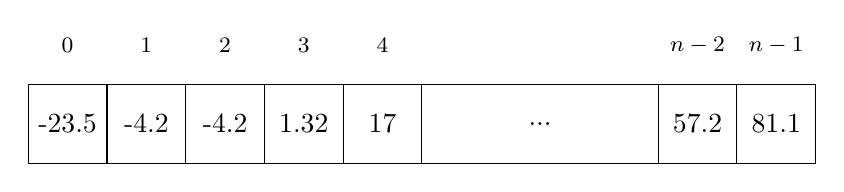
\begin{tikzpicture}
%\node[minimum size=1cm,draw] at (-1.5,0) {6};
%\node[minimum size=1cm,draw] at (-3,0) {8};
%\node at (-1.5,1) {\rotatebox{45}{size}};
%\node at (-2.7,1.2) {\rotatebox{45}{capacity}};

\node[minimum size=1cm,draw] at (0,0) {-23.5};
\node[minimum size=1cm,draw] at (1,0) {-4.2};
\node[minimum size=1cm,draw] at (2,0) {-4.2};
\node[minimum size=1cm,draw] at (3,0) {1.32};
\node[minimum size=1cm,draw] at (4,0) {17};
\node[minimum size=1cm,minimum width=3cm,draw] at (6,0) {...};
\node[minimum size=1cm,draw] at (8,0) {57.2};
\node[minimum size=1cm,draw] at (9,0) {81.1};

\node at (0,1) {\footnotesize 0};
\node at (1,1) {\footnotesize 1};
\node at (2,1) {\footnotesize 2};
\node at (3,1) {\footnotesize 3};
\node at (4,1) {\footnotesize 4};
\node at (8,1) {\footnotesize $n-2$};
\node at (9,1) {\footnotesize $n-1$};
\end{tikzpicture}


\end{document}
